
\section{System Overview}

In this section, we introduce the main components of the system. Our system is 
built with a pipeline architecture in mind giving it the advantage to run 
each section separately to allow stream processing without blocking the data flow of components 
(Figure~\ref{fig:system}).
The three logical components include sections for performing preprocessing to prepare the required data, 
Cumulative Citation Recommendation to annotate cite-worthy documents, Streaming 
Slot Filling to generate the actual slot values and PostProcessing to 
increase precision/recall. 
TREC provides a streaming data set and  entities from Twitter or WP to query.

%\ceg{Discuss current system first. If you want to keep the decisions points that led to the current architecture, make it a subsection.}

\begin{figure}
  \centering
%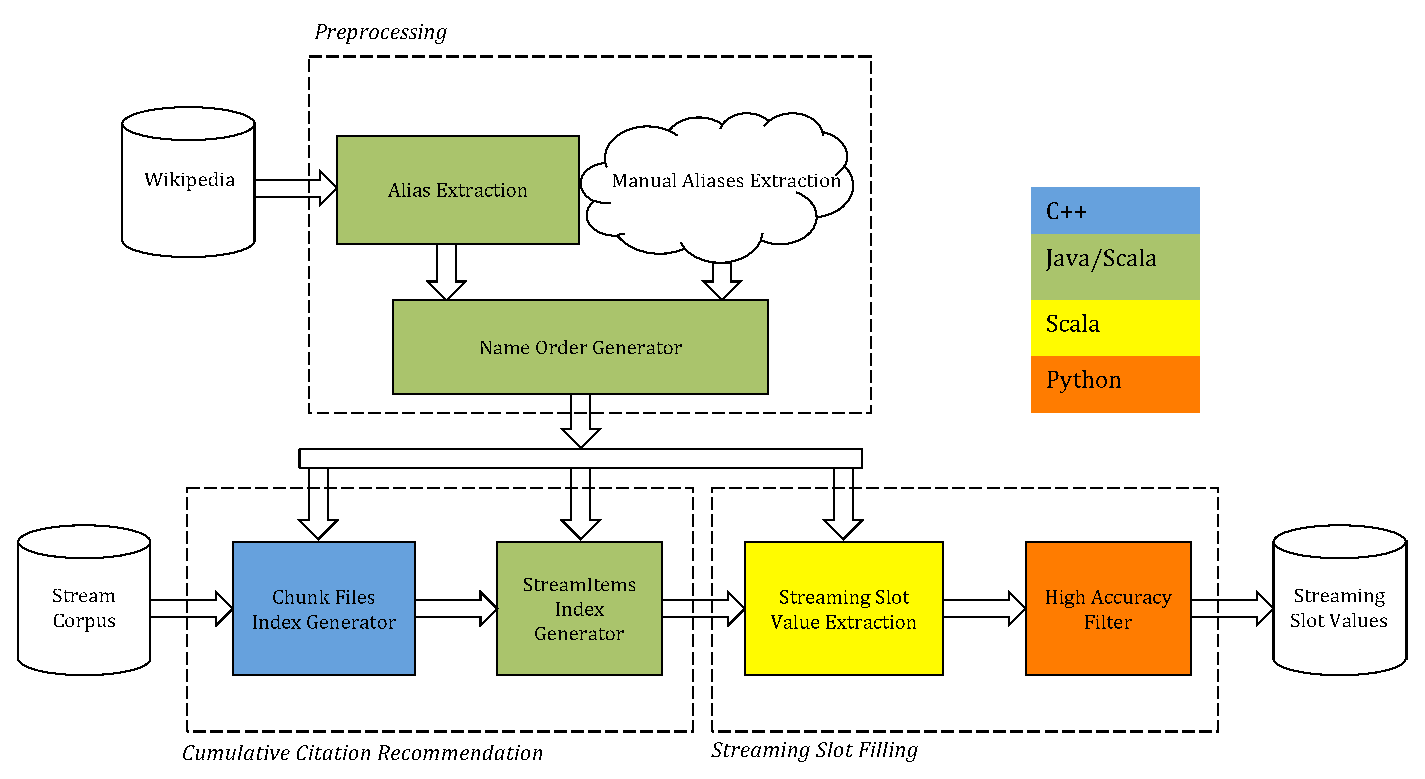
\includegraphics[width=6in]{./images/sdl.eps}
  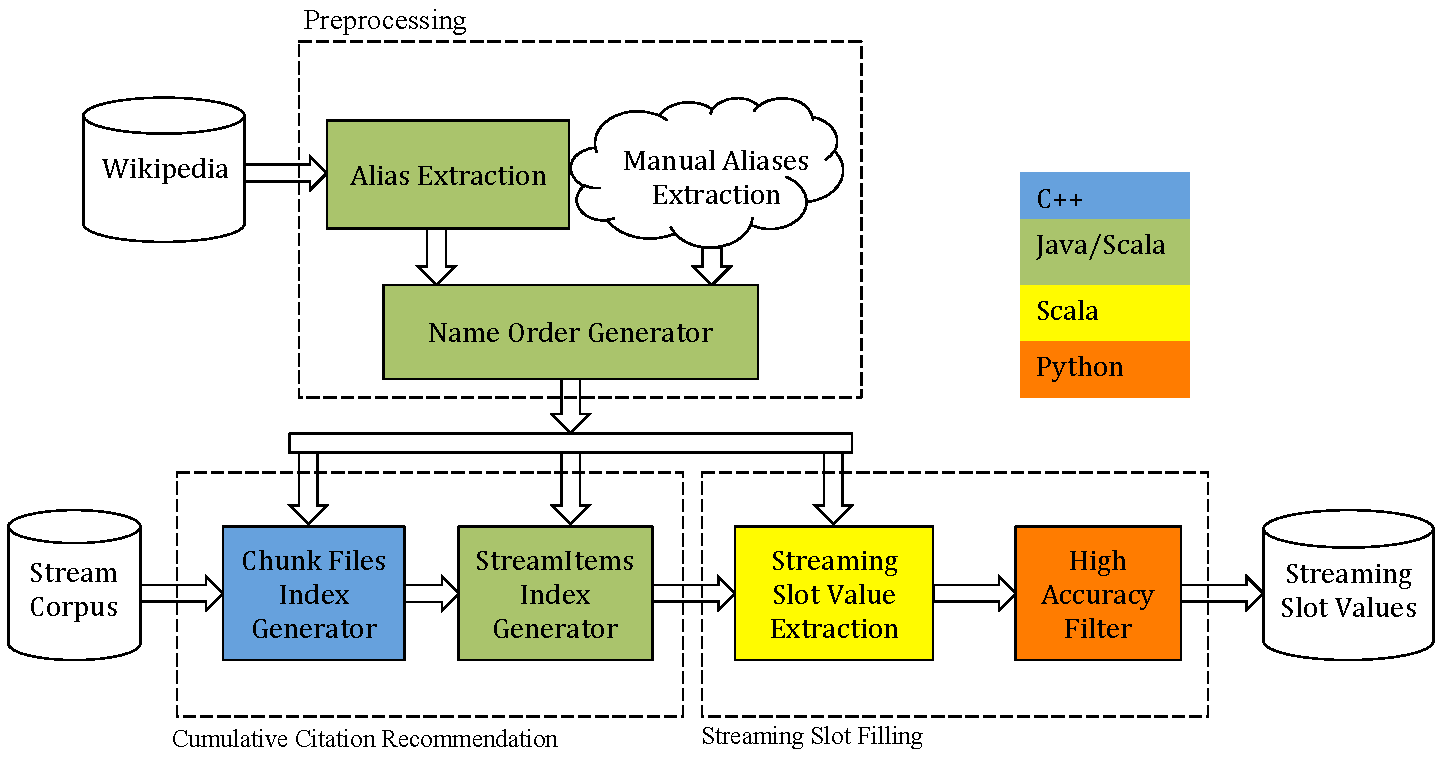
\includegraphics[width=6in]{./images/System_Diagram_Languages.pdf}
% http://convert.neevia.com/pdfconvert/
  \vspace*{-.1in} 
  \caption{The GatorDSR team System Architecture.
  Components are logically groups with dotted boxes.
  Color details the programing language implementation of components.}
  \label{fig:system}
  \vspace*{-.2in}
\end{figure}



\textbf{Preprocessing.}
\label{sec:preproc}
The contest prohibits Wikipedia entities to have any manual aliases being added and only
allows automatic ways. We use Wikipedia API backlink references
(redirects to a wiki entity) as aliases of the entity. We also extract 
aliases from within the text of a wiki entity, which will be described in
Section~\ref{section:aliasgeneration}. This whole process is referred to as
\textit{Alias Extraction}. 
The manual extraction rule is lifted and participants are allowed to manually add aliases for Twitter entities.
This is allowed because the Twitter website does not provide an example page from the beginning of the document stream.
This process of extracting
aliases for Twitter entities is referred to as \textit{Manual Alias Extraction}.

Once aliases are available we pass them through rules of generating proper name 
orders which will produce various forms of writing a name. As a basic example Bill 
Gates can be written as Gates, Bill. This will allow the system to capture various 
notation forms of aliases. We refer to this part as \textit{Name Order Generator}.

\textbf{Cumulative Citation Recommendation.}
\label{sec:ccr1}
The main goal of CCR is to have an aggregate list of documents that are worthy of being cited in a Wikipedia page. We perform exact string matching 
and treat all the documents that mention an entity equally likely to be citable. One of the reasons for this is 
that in former TREC KBA reports \cite{JFrank12} there were observations of how 
non-mentioning documents have a low chance of being citable in Wikipedia.
So we take on that and ignore non-citing documents. 


% Note: Describe the algorithms of each phase
% Talk in abstract terms not implementation.
% Use formal representations (Math, SQL etc)


%\ceg{This section should be structured as follows:
%1: Introduce CCR (Motivation, Expectations)
%2: Our high level approach
%3: Discussion of our design (Like already discussed)
%}


\textbf{Streaming Slot Filling.}
\label{sec:ssf1}
%\ceg{See the previous note.}
The purpose of SSF is to extract proper values for relations of
interest, which can be found in Table~\ref{table:slotNameOntology}.
This is called Stream Slot Filling because data is being generated as time goes
on and for each extraction we should only consider current or past data.
In Figure~\ref{fig:system} we refer to this as \textit{Streaming Slot Value Extraction}.
Stream slot filling is done by pattern matching documents with manually 
produced patterns for slots of interest. The way we do this is by observing a 
sentence that has a mention of the entity or one of its coreferences. An 
anchor word in the sentence related to the slot name is located and we match 
either left or right of the anchor word for potential slot values. 

\textbf{Post Processing Algorithm.}
\label{sec:postproc}
The SSF output of many extractions is noisy. The data contains duplicates and 
incorrect extractions. We can define rules to sanitize the output only using 
the information present in the SSF file. The file is processed in time order, 
in a tuple-at-a-time fashion to minimize the impact on accuracy. We define 
two classes of rules deduplication rules and inference rules. In our diagram we refer to this component as \textbf{High Accuracy Filter}.
